%\documentclass[a4paper,handout]{beamer}
\documentclass[presentation]{beamer}
%\usepackage[francais]{babel}
\usepackage[utf8]{inputenc}
\usetheme{Inuits}
\usepackage[T1]{fontenc}
\usepackage{listings}
\usepackage{eso-pic}
\setbeamercolor{background canvas}{bg=} 
\definecolor{inuitstitle}{RGB}{153,153,255}
\definecolor{inuitsgreen}{RGB}{35,255,35}
\usecolortheme[RGB={90,90,149}]{structure} 
\usebackgroundtemplate{%

\includegraphics[height=\paperheight,widht=\paperwidth]{files/background.png};}

%\AddToShipoutPicture{\put(0,5){%
%   \parbox[b][\paperheight]{\paperwidth}{%
%     \vfill
%     \centering
%     \rotatebox{0}{
\includegraphics[width=\paperwidth,height=\paperheight,%
%                      ]{files/background.png}}%
%     \vfill
%}}}
\setbeamercolor{normal text}{fg=white}
\setbeamercolor{block body}{fg=black}
\setbeamercolor{itemize item}{fg=inuitsgreen}
\setbeamercolor{itemize subitem}{fg=inuitsgreen}
\setbeamercolor{itemize subitem subitem}{fg=inuitsgreen}
\setbeamertemplate{itemize item}[circle] 
\setbeamertemplate{itemize subitem}[circle] 
\setbeamertemplate{sections/subsections in toc}[circle]

%\setbeamercolor{palette primary}{fg=inuitstitle,bg=black!85}
%\setbeamercolor{palette secondary}{fg=white,bg=inuitstitle}
%\setbeamercolor{palette tertiary}{fg=white,bg=black!85}
%\setbeamercolor{palette quaternary}{fg=inuitstitle}
%\setbeamercolor{block title}{fg=inuitstitle}
%\setbeamercolor{sidebar}{bg=inuitstitle!70}

%\AtBeginDocument{%
%    \pgfdeclareverticalshading{beamer@topshade}{\paperwidth}{%
%      color(0pt)=(bg);
%      color(4pt)=(black)}
%}


\setbeamercolor{title}{fg=inuitstitle,bg=}

\setbeamertemplate{navigation symbols}{}
\definecolor{OliveGreen}{RGB}{0,100,0}
\definecolor{grey}{RGB}{150,150,150}
\definecolor{darkgrey}{RGB}{100,100,100}
\definecolor{inuits}{RGB}{153,153,255}
\usepackage{shadowtext}
\newcommand{\xitem}[1]{\item{\shadowtext{#1}}}
\newcommand{\inuits}[1]{\shadowtext{\color{inuits}#1}}

\begin{document}
\setbeamercovered{invisible}

\title[Monitoring at Cloud Scale]{\fontsize{25}{35}\selectfont Monitoring at Cloud Scale}

\author[Julien Pivotto]{\shadowtext{Julien Pivotto}}
\institute[Inuits]{
\includegraphics[height=2cm]{files/inuitslogo.png}}
\date{\shadowtext{Build a cloud Day Amsterdam}\\\inuits{June 13th, 2013}}
\logo{
\includegraphics[height=1cm]{files/bacd.png}}

\frame[plain]{\titlepage}

\frame{%
\frametitle{Table of contents}
\tiny
\tableofcontents
}

\frame{%
    \begin{center}\begin{Huge}{\inuits{Julien Pivotto}}\end{Huge}\end{center}
    \begin{large}
    \begin{itemize}
        \xitem{sysadmin @ inuits}
        \xitem{open-source defender for 7+ years}
        \xitem{devops believer}
        \xitem{@roidelapluie on twitter/github}
    \end{itemize}
    \end{large}
}
\section{Introduction}
\subsection{DevOps}
\frame{%
    \frametitle{What is that DevOps stuff again?}
    \begin{columns}[T]
        \begin{column}{.5\textwidth}
            \begin{LARGE}
                \begin{itemize}
                    \xitem{Culture}
                    \xitem{\textit{(Lean)}}
                    \xitem{Automation}
                    \xitem{\color{inuits}{Measurement}}
                    \xitem{Sharing}
                \end{itemize}
            \end{LARGE}
        \end{column}
        \begin{column}{.5\textwidth}
            
\includegraphics[height=3cm]{files/devops.png}
            \vspace{1.5cm}
            \begin{flushright}\textit{\inuits{Damon Edwards and John Willis}}\end{flushright}
        \end{column}
    \end{columns}
}


\subsection{monitoringsucks}
\frame{%
    \frametitle{\#monitoringsucks}
    \begin{large}
    \begin{itemize}
        \xitem{https://github.com/monitoringsucks}
        \xitem{a movement to find a solution to monitoring}
        \xitem{the feeling that monitoring is stucked in the past}
    \end{itemize}
    \end{large}
}

\subsection{monitoringsucks}
\frame{%
    \frametitle{\#monitoringlove}
    \begin{LARGE}
    \begin{itemize}
        \xitem{then it turned into \color{inuits}{\#monitoringlove}}
        \xitem{relevant tools exist}
        \xitem{they just need to be used}
        \xitem{following the unix philosophy}
    \end{itemize}
    \end{LARGE}
    \begin{flushright}\textit{\inuits{we are going to explore some of them}}\end{flushright}
}
\section{Around monitoring}
\subsection{The cloud}
\frame{%
    \frametitle{What is different in the cloud?}
    \begin{huge}
    \begin{itemize}
        \xitem{Scale}
        \xitem{Velocity}
        \xitem{More changes, more often}
    \end{itemize}
    \end{huge}
}
\frame{%
    \frametitle{What do you need?}
    \begin{huge}
    \begin{itemize}
        \xitem{scalability}
        \xitem{automation}
    \end{itemize}
    \end{huge}
}
\subsection{The past}

\frame{%
    \frametitle{time for retirement}
    \begin{huge}
    \begin{itemize}
        \xitem{forget all-in-one tools}
        \xitem{forget auto-discovery tools}
        \xitem{forget non-scalable tools}
        \xitem{forget tools you can not automate}
    \end{itemize}
    \end{huge}
}

\frame{%

    \frametitle{forget about\ldots}
    \flushright{\tiny{\color{darkgrey}http://www.flickr.com/photos/mourner/150844753/}}
    \begin{center}
        
\includegraphics[height=5cm]{files/flickr_graveyard.jpg}\\
        \only<1>{\huge{\shadowtext{Zabbix}}}
        \only<2>{\huge{\shadowtext{Centreon}}}
        \only<3>{\huge{\shadowtext{GroundWork}}}
        \only<4>{\huge{\shadowtext{Cacti}}}
        \only<5>{\huge{\shadowtext{Hyperic}}}
        \only<6>{\huge{\shadowtext{BigBrother}}}
        \only<7>{\huge{\shadowtext{Munin}}}
        \only<8>{\huge{\shadowtext{Zenoss}}}
    \end{center}

}

\subsection{Environment}
\frame{%
    \frametitle{Your infrastructure today}
    \flushright{\tiny{\color{darkgrey}http://www.flickr.com/photos/bjbrake/235217140/}}
    \begin{center}
        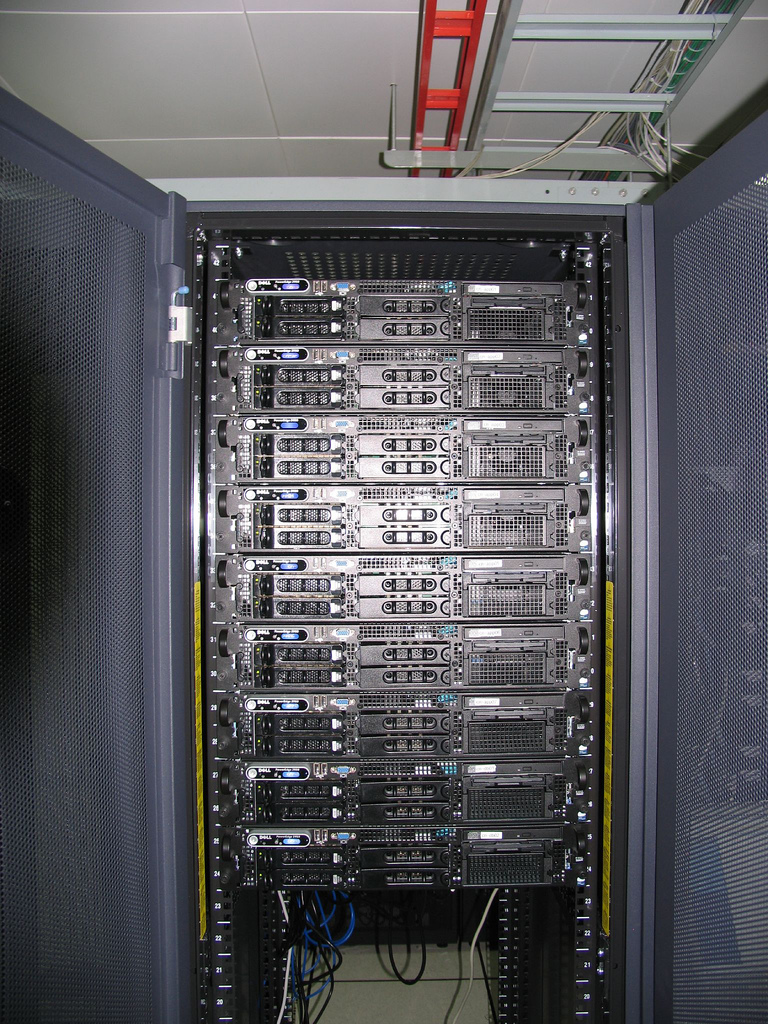
\includegraphics[height=6cm]{files/flickr_rack.jpg}
    \end{center}
}
\frame{%
    \frametitle{Your infrastructure tomorrow}
    \flushright{\tiny{\color{darkgrey}http://www.flickr.com/photos/bjbrake/235217140/}}
    \begin{center}
        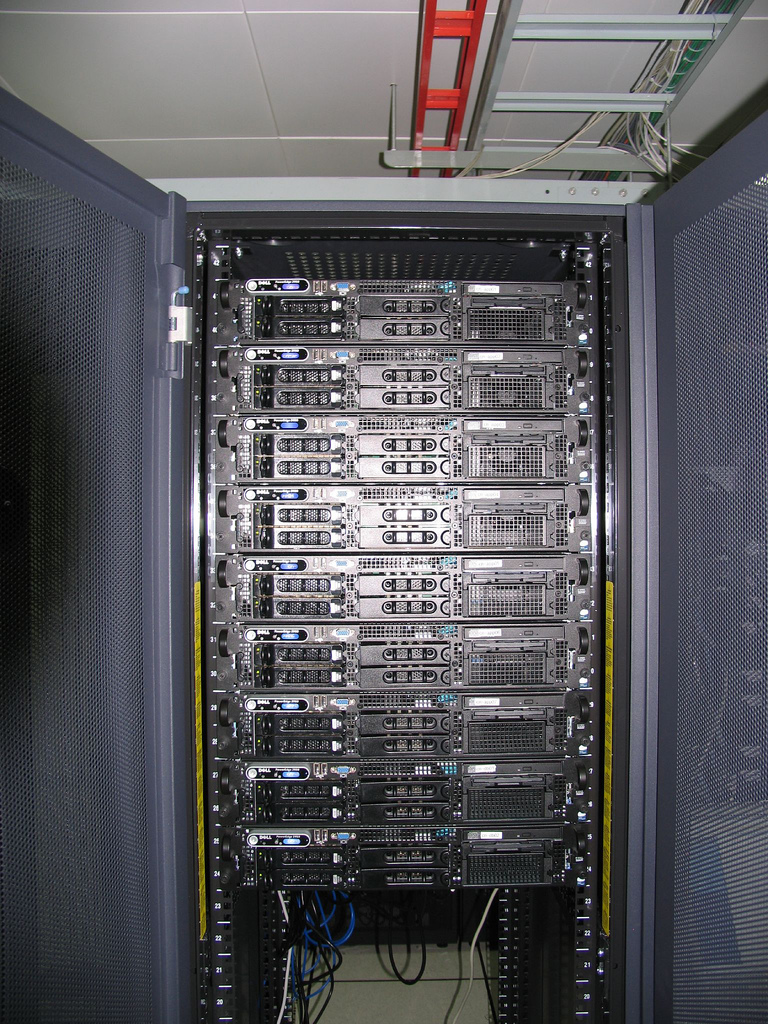
\includegraphics[height=6cm]{files/flickr_rack.jpg}
        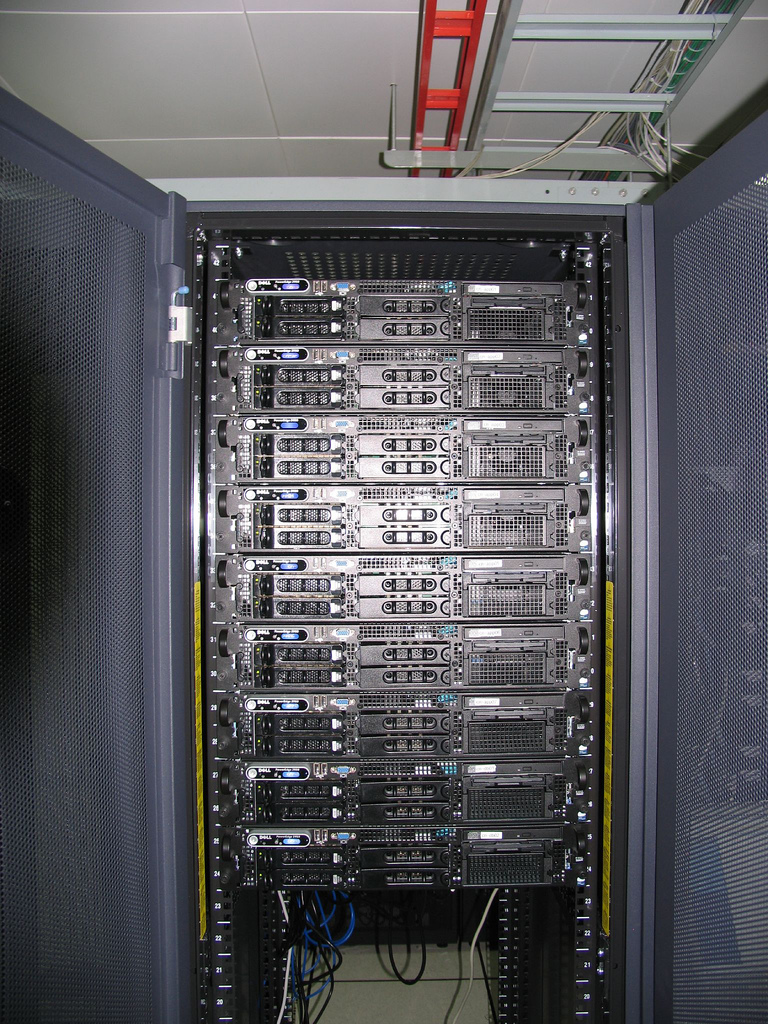
\includegraphics[height=6cm]{files/flickr_rack.jpg}
    \end{center}
}
\frame{%
    \frametitle{Your infrastructure in 6 months}
    \flushright{\tiny{\color{darkgrey}http://www.flickr.com/photos/bjbrake/235217140/}}
    \begin{center}
        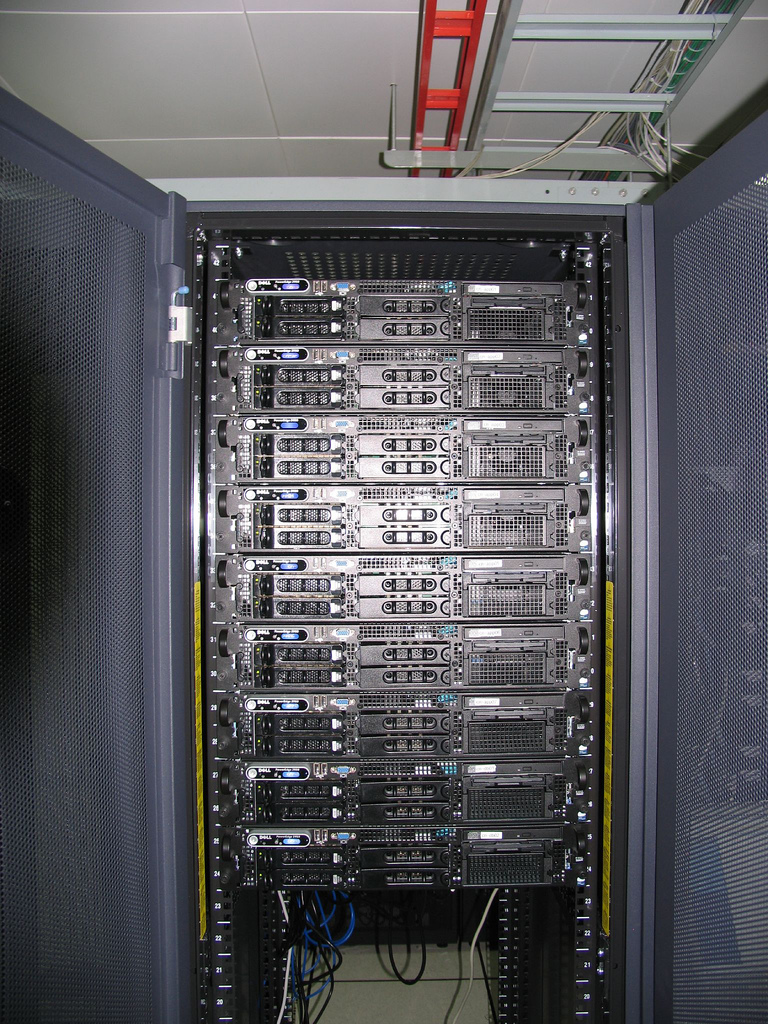
\includegraphics[height=1.5cm]{files/flickr_rack.jpg}
        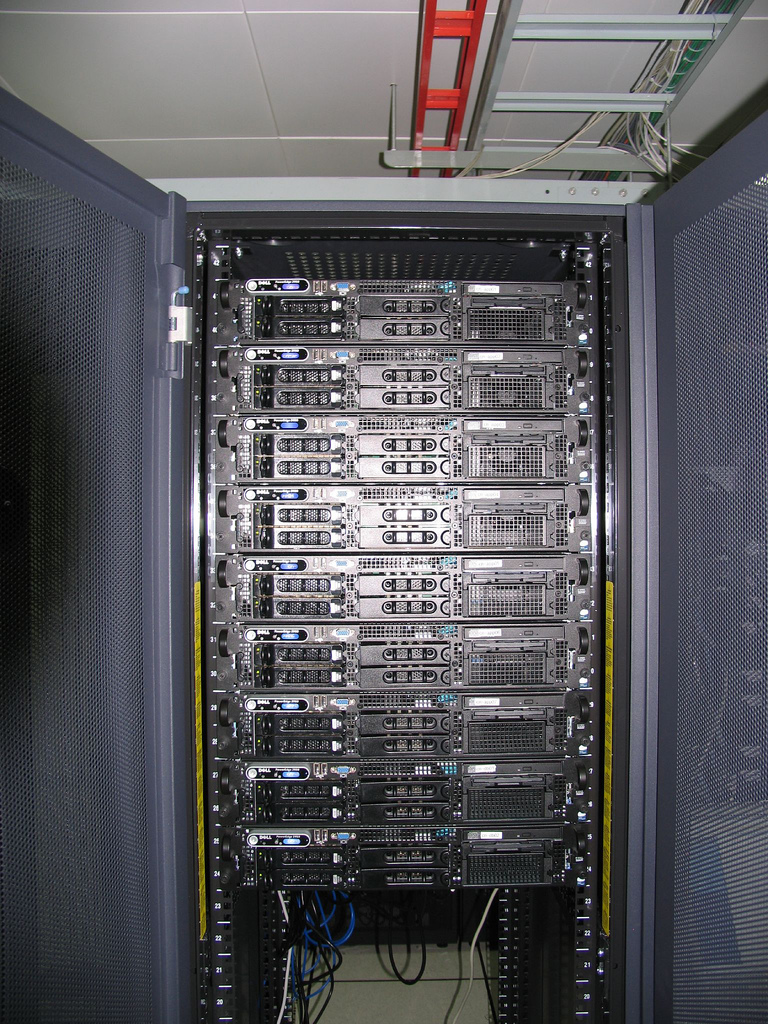
\includegraphics[height=1.5cm]{files/flickr_rack.jpg}
        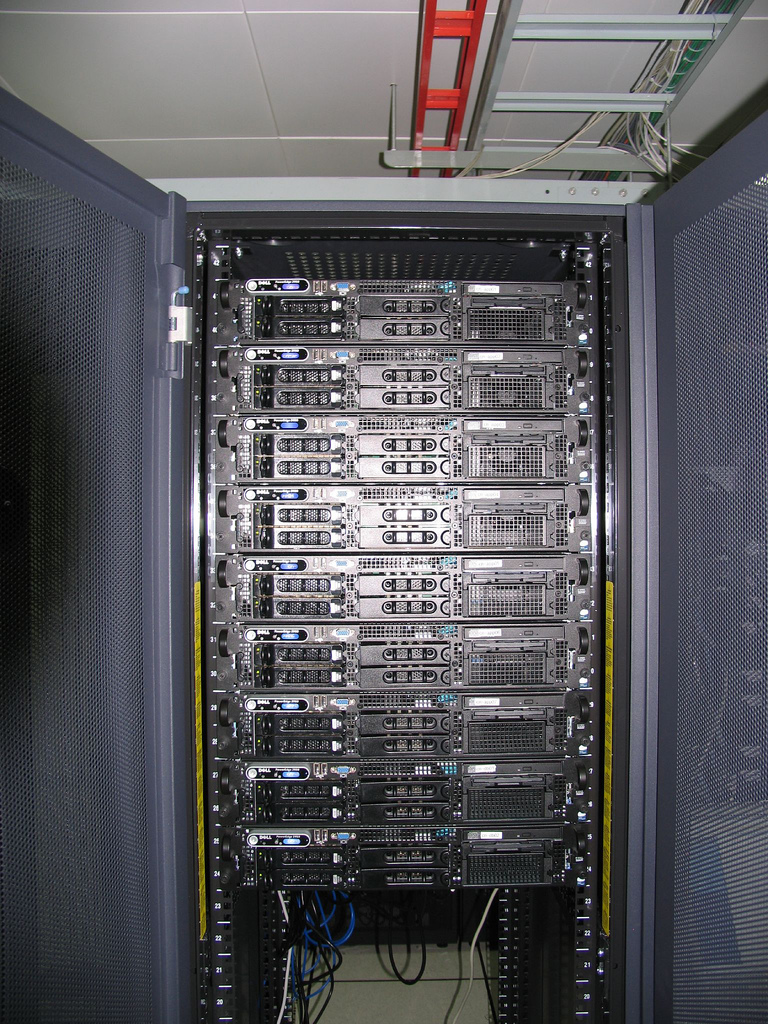
\includegraphics[height=1.5cm]{files/flickr_rack.jpg}
        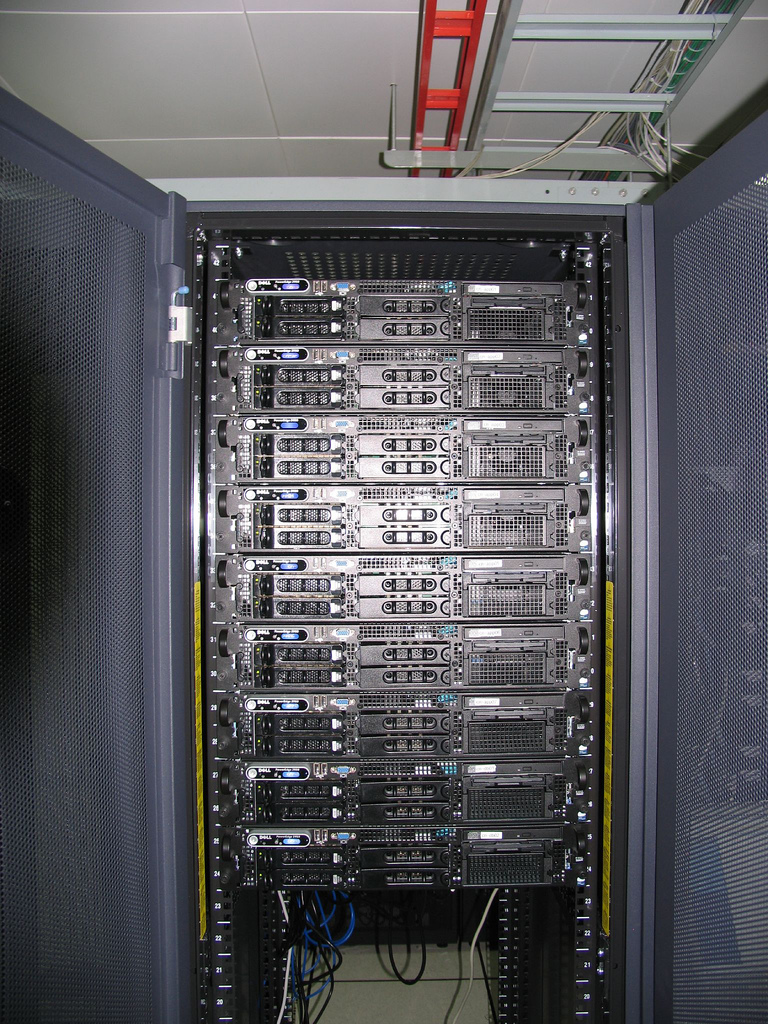
\includegraphics[height=1.5cm]{files/flickr_rack.jpg}
        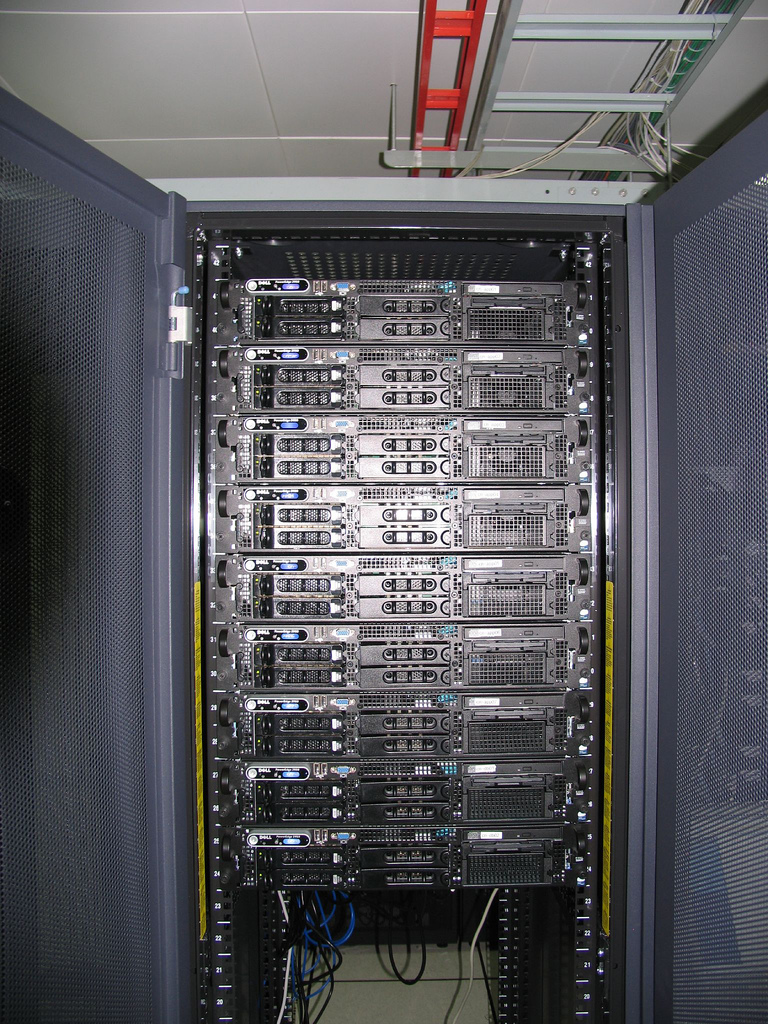
\includegraphics[height=1.5cm]{files/flickr_rack.jpg}
        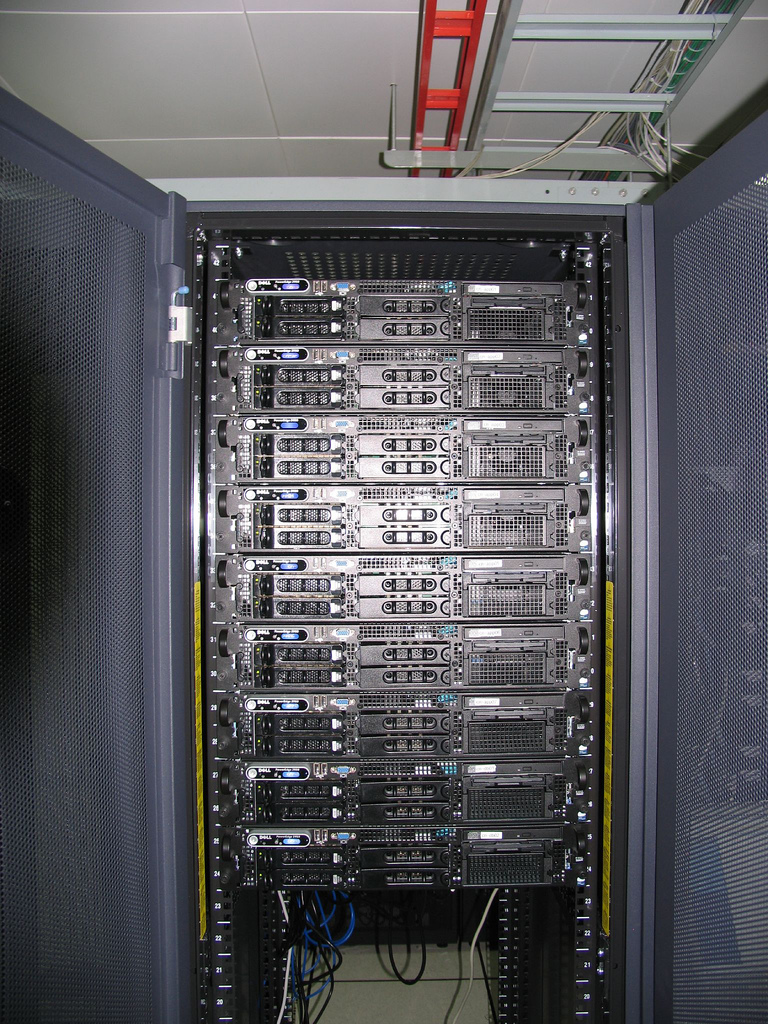
\includegraphics[height=1.5cm]{files/flickr_rack.jpg}\\
        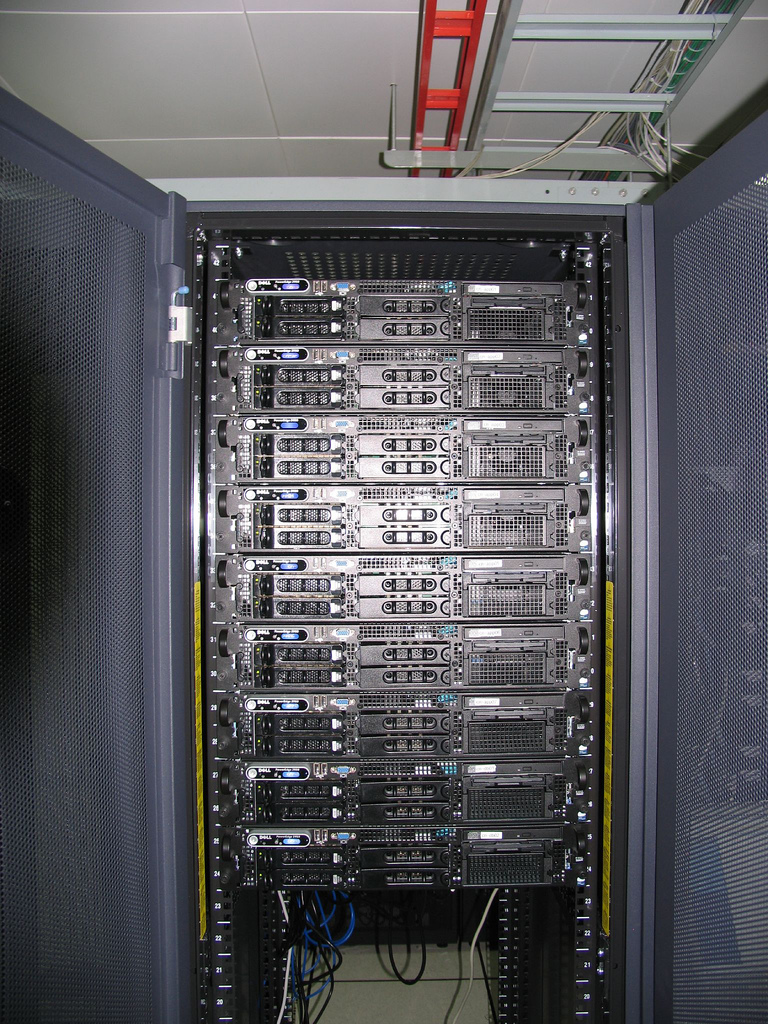
\includegraphics[height=1.5cm]{files/flickr_rack.jpg}
        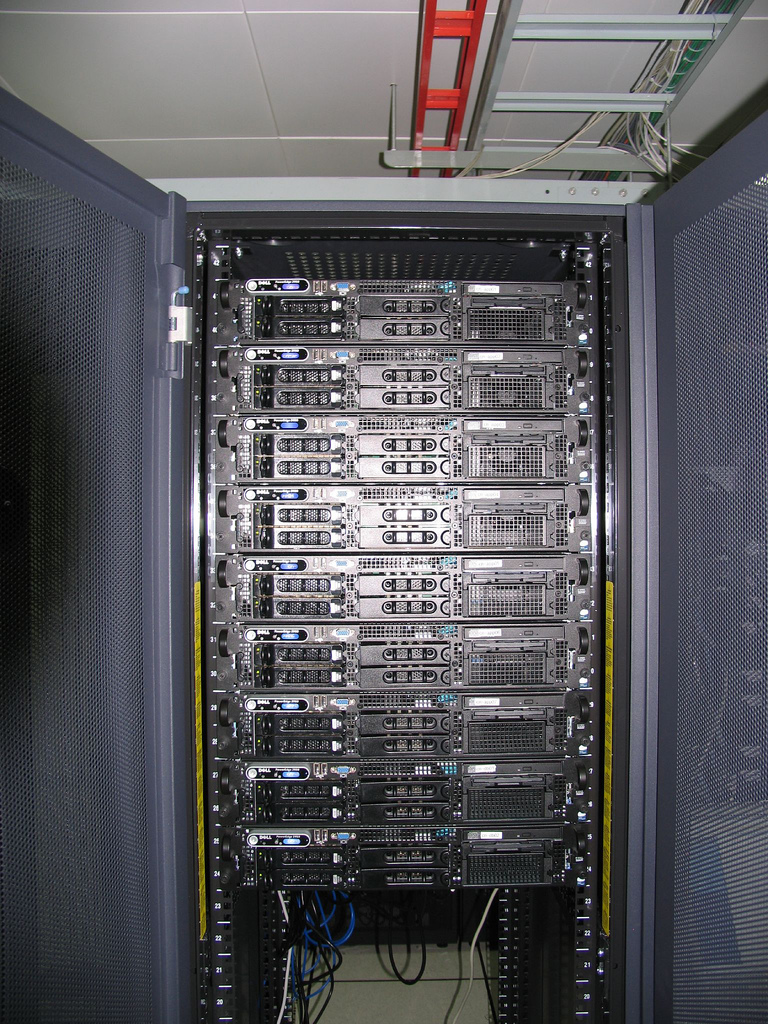
\includegraphics[height=1.5cm]{files/flickr_rack.jpg}
        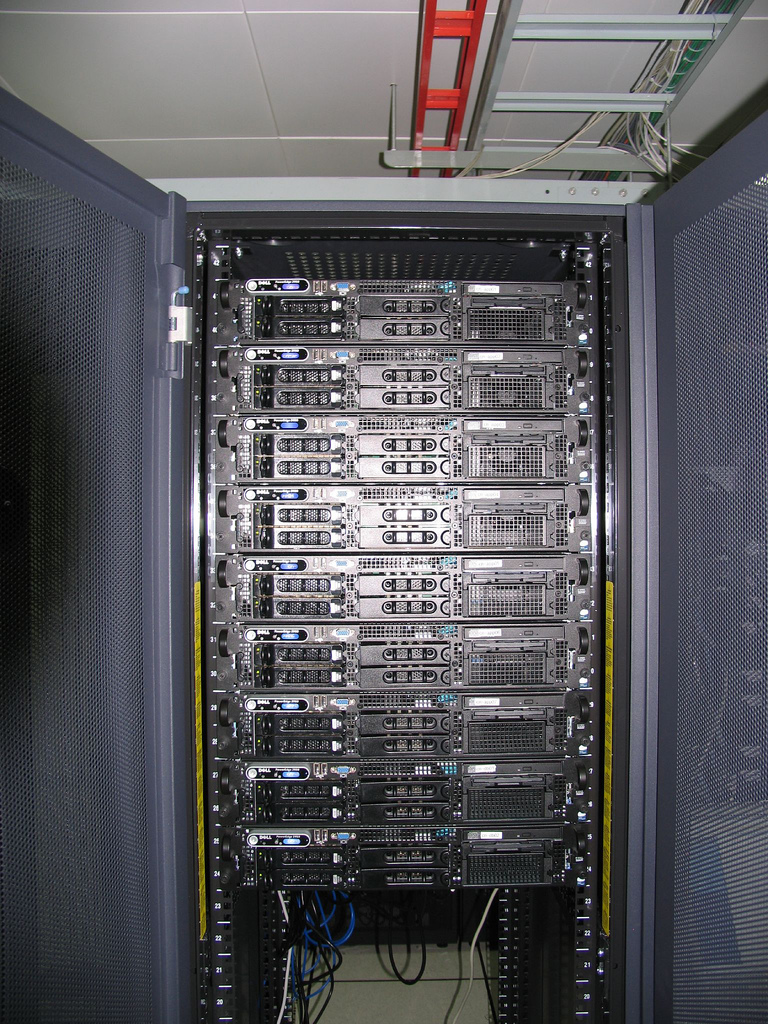
\includegraphics[height=1.5cm]{files/flickr_rack.jpg}
        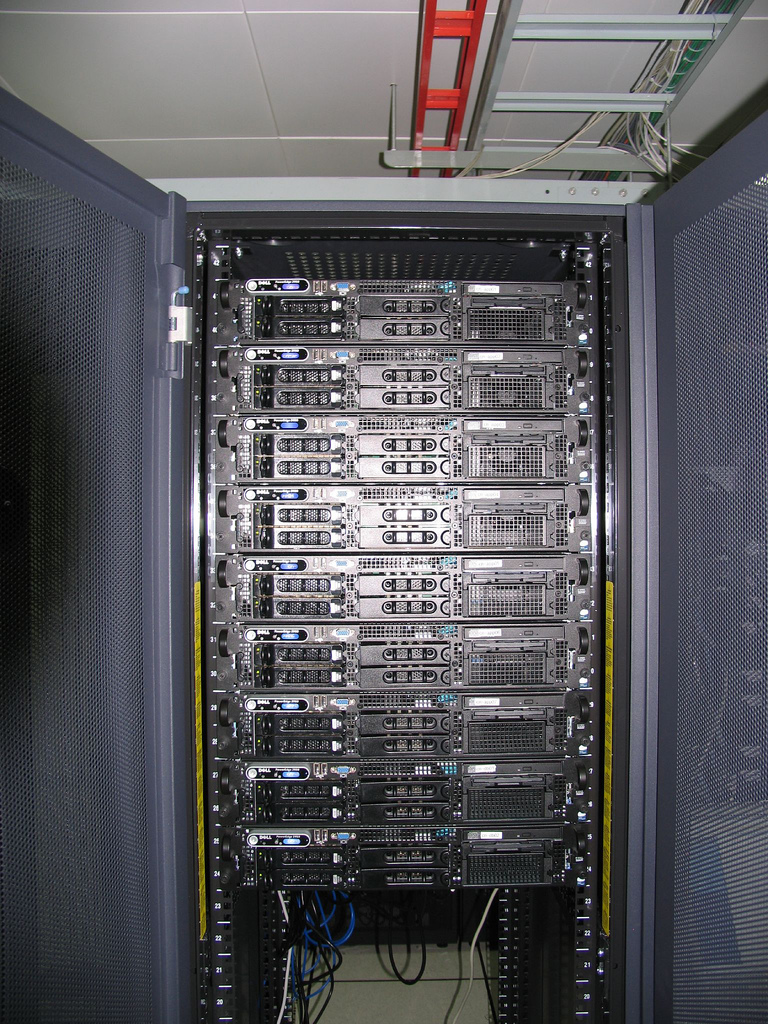
\includegraphics[height=1.5cm]{files/flickr_rack.jpg}
        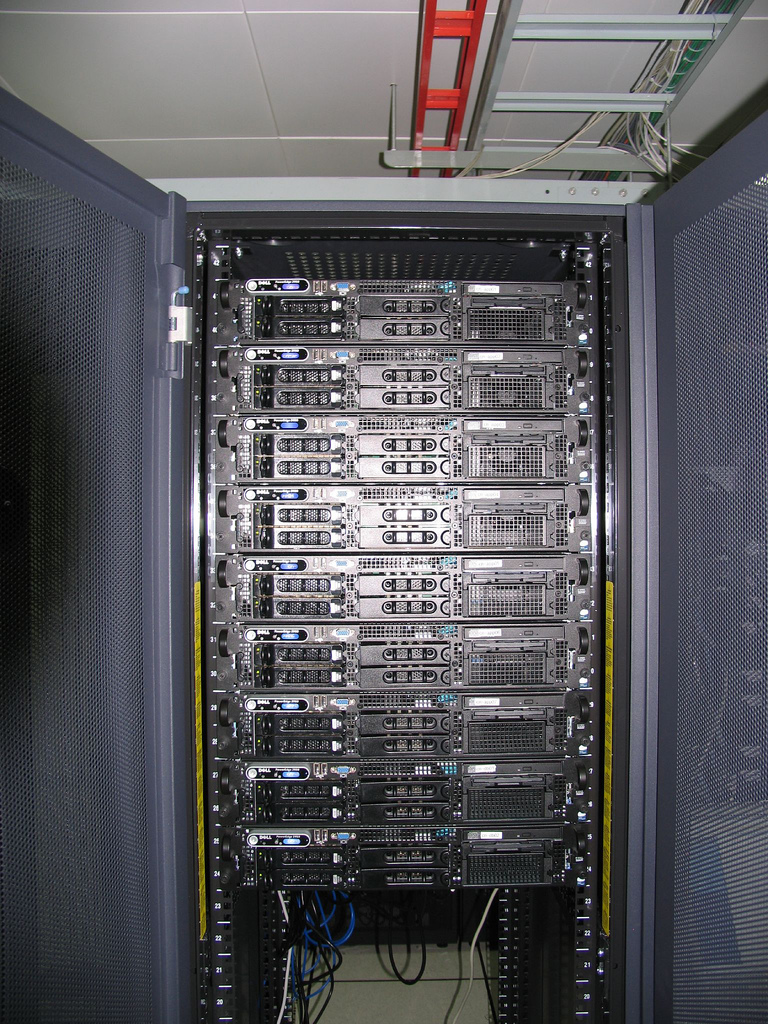
\includegraphics[height=1.5cm]{files/flickr_rack.jpg}
        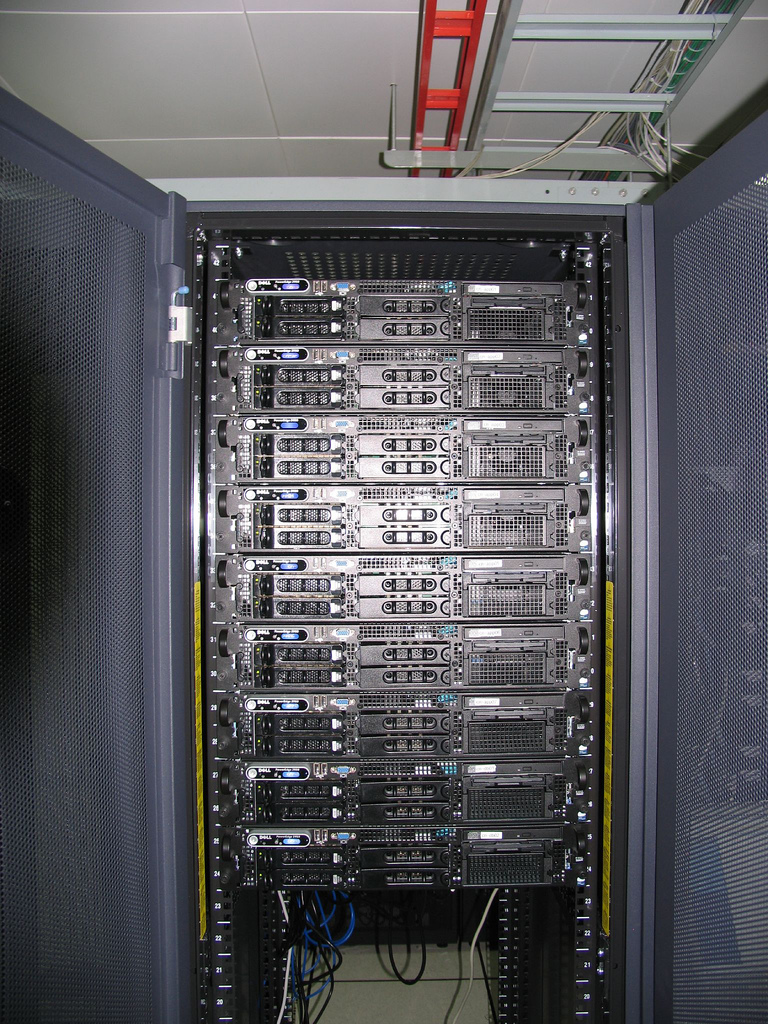
\includegraphics[height=1.5cm]{files/flickr_rack.jpg}\\
        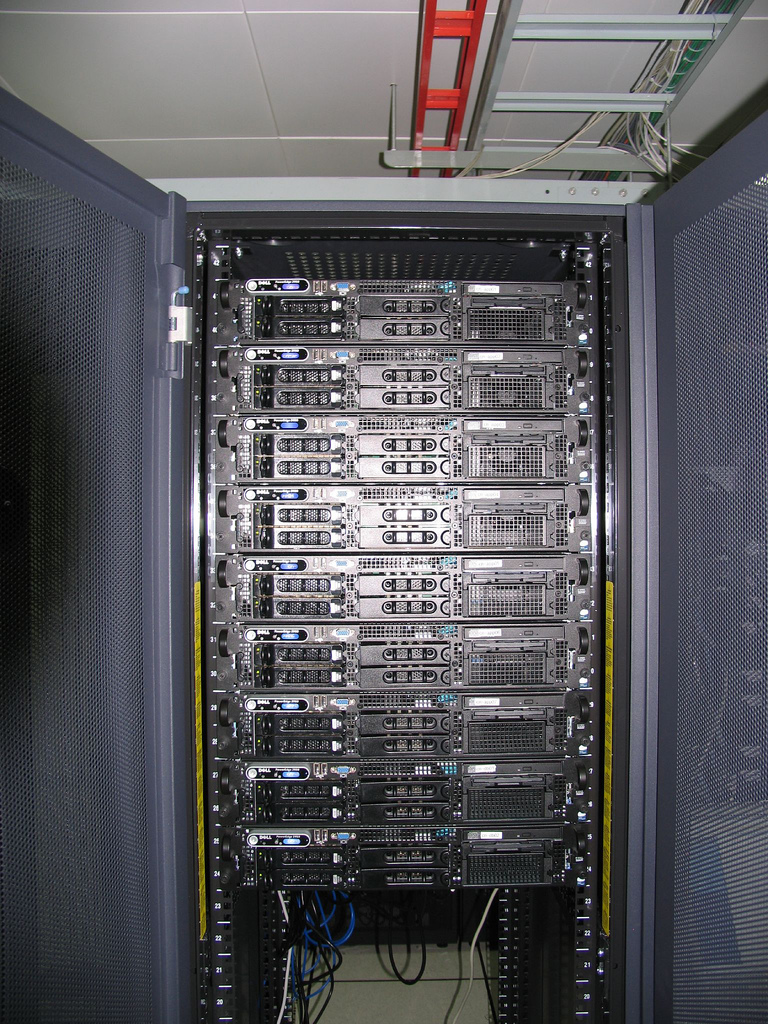
\includegraphics[height=1.5cm]{files/flickr_rack.jpg}
        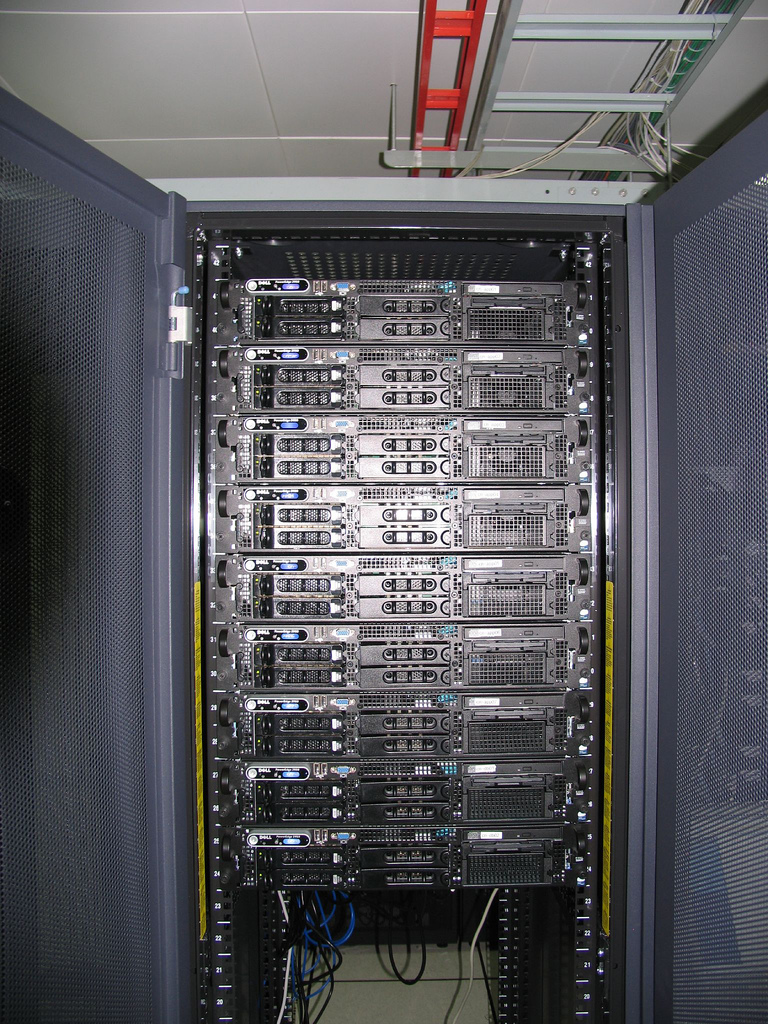
\includegraphics[height=1.5cm]{files/flickr_rack.jpg}
        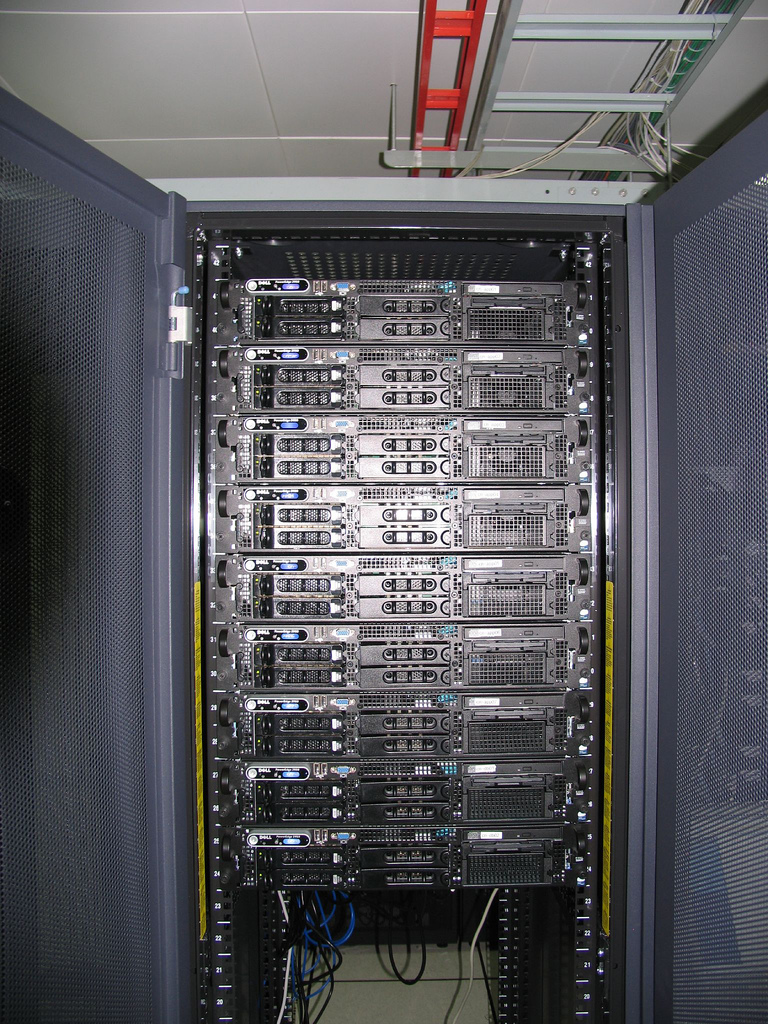
\includegraphics[height=1.5cm]{files/flickr_rack.jpg}
        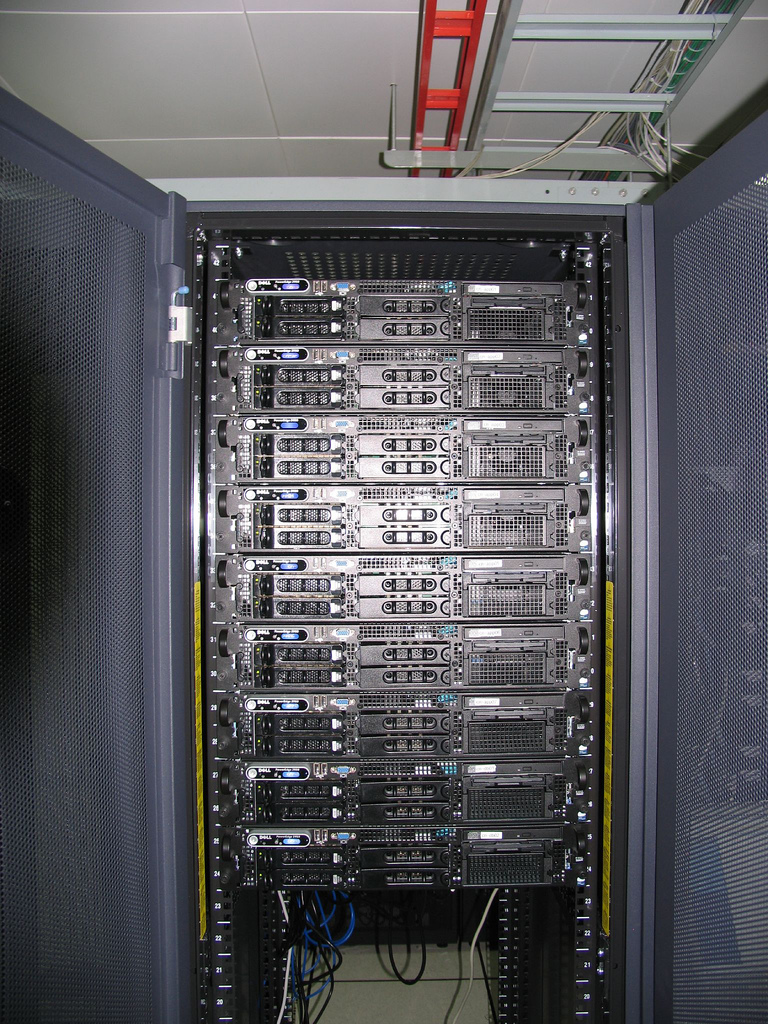
\includegraphics[height=1.5cm]{files/flickr_rack.jpg}
        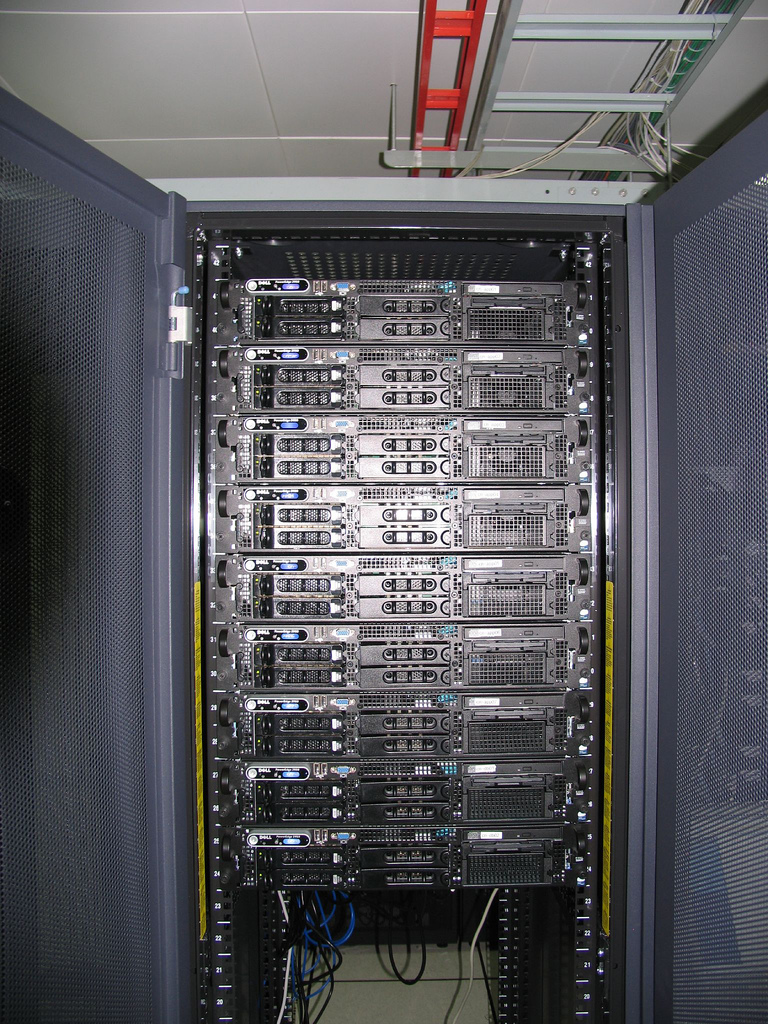
\includegraphics[height=1.5cm]{files/flickr_rack.jpg}
        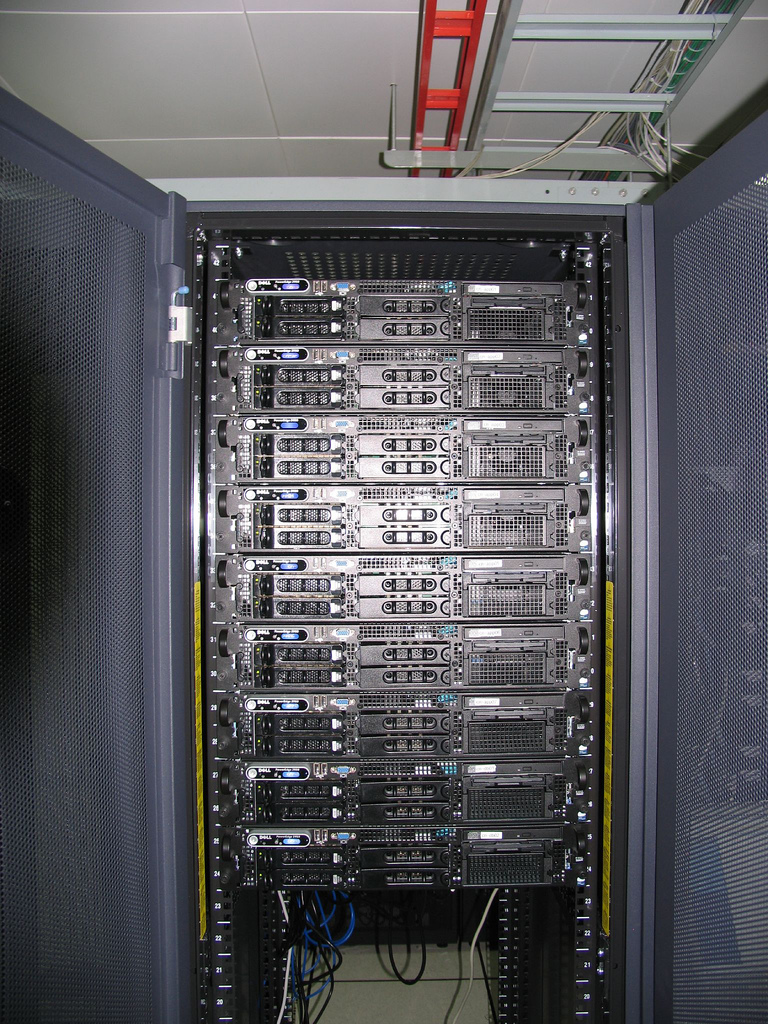
\includegraphics[height=1.5cm]{files/flickr_rack.jpg}\\
        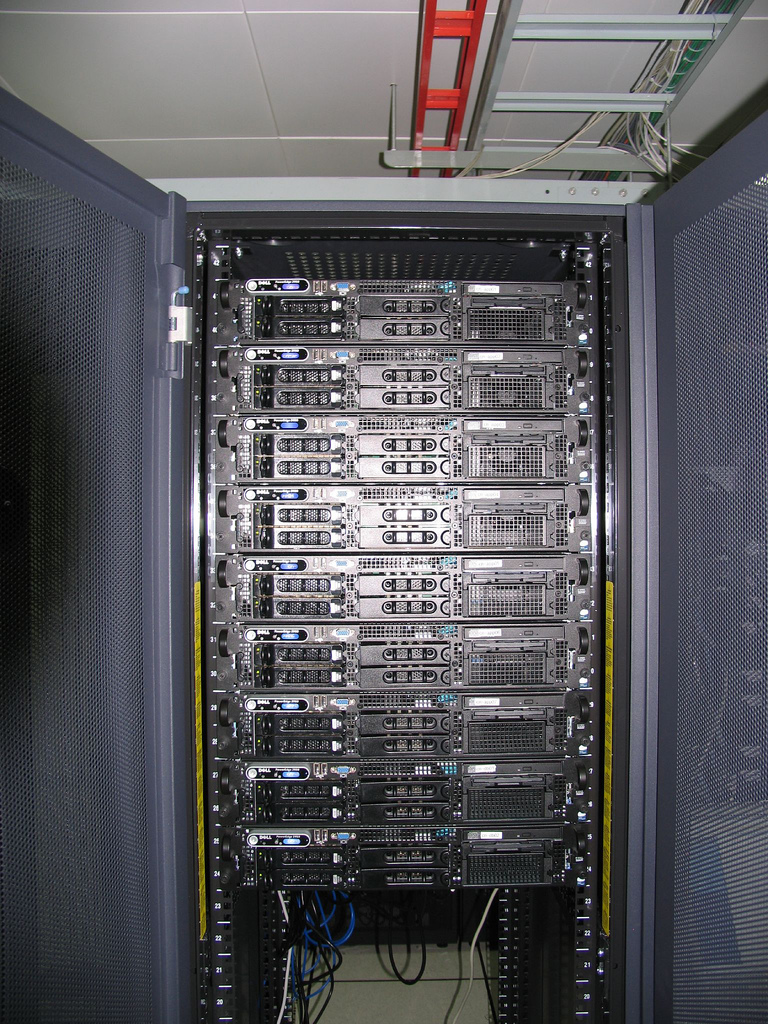
\includegraphics[height=1.5cm]{files/flickr_rack.jpg}
        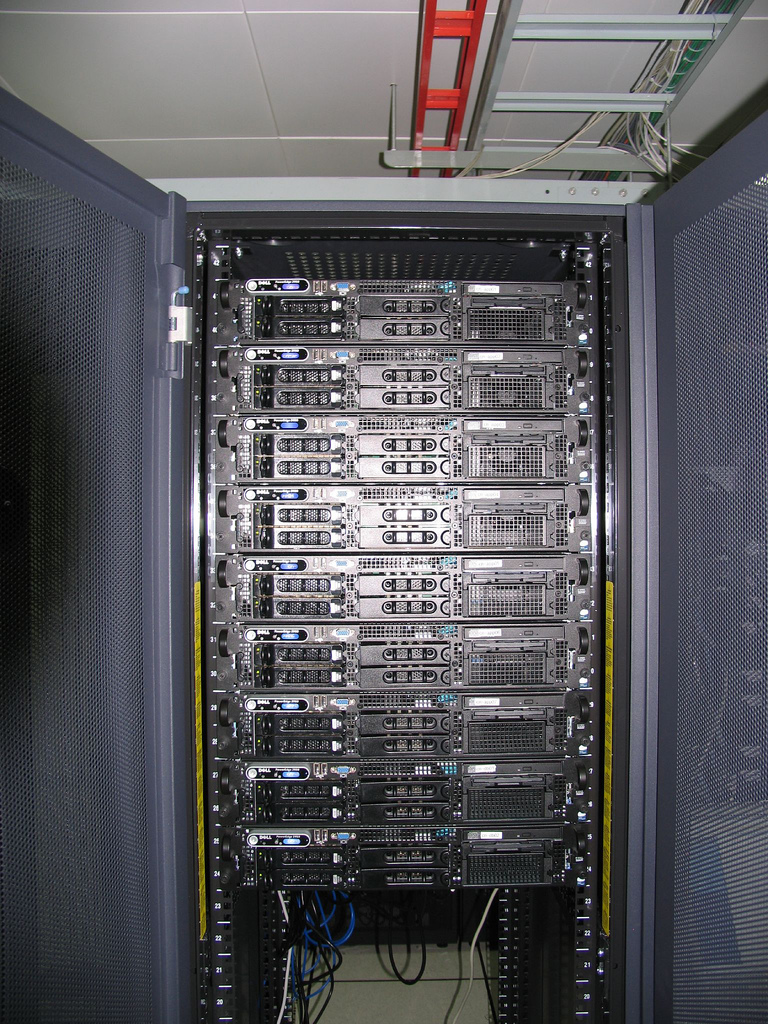
\includegraphics[height=1.5cm]{files/flickr_rack.jpg}
        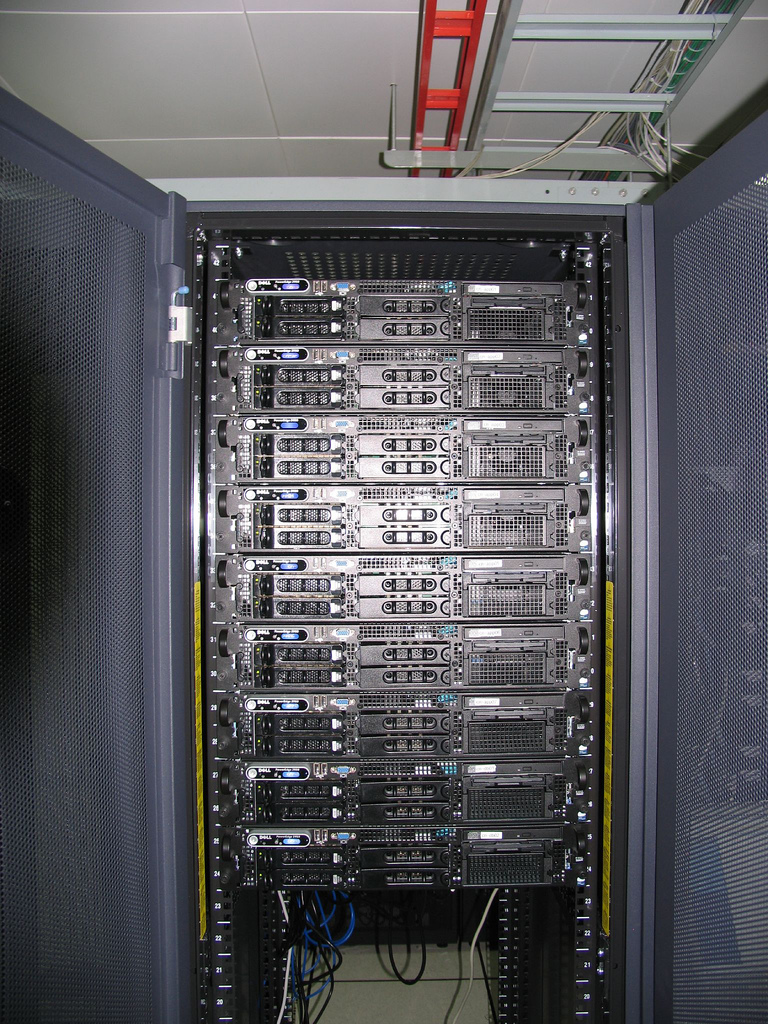
\includegraphics[height=1.5cm]{files/flickr_rack.jpg}
        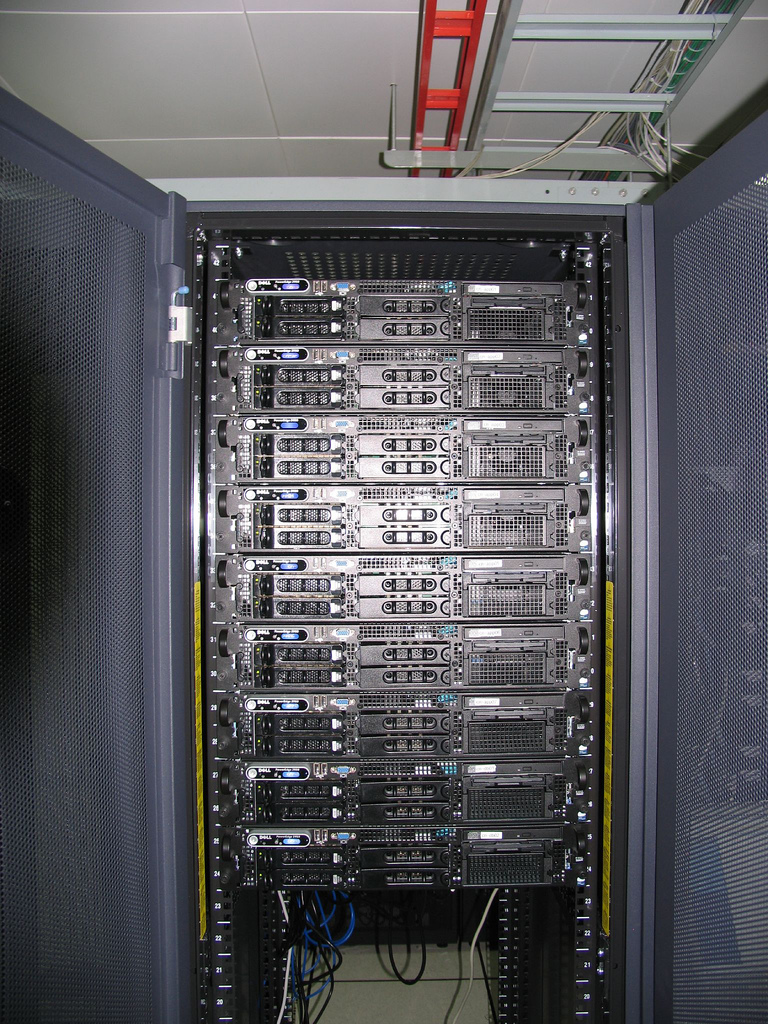
\includegraphics[height=1.5cm]{files/flickr_rack.jpg}
        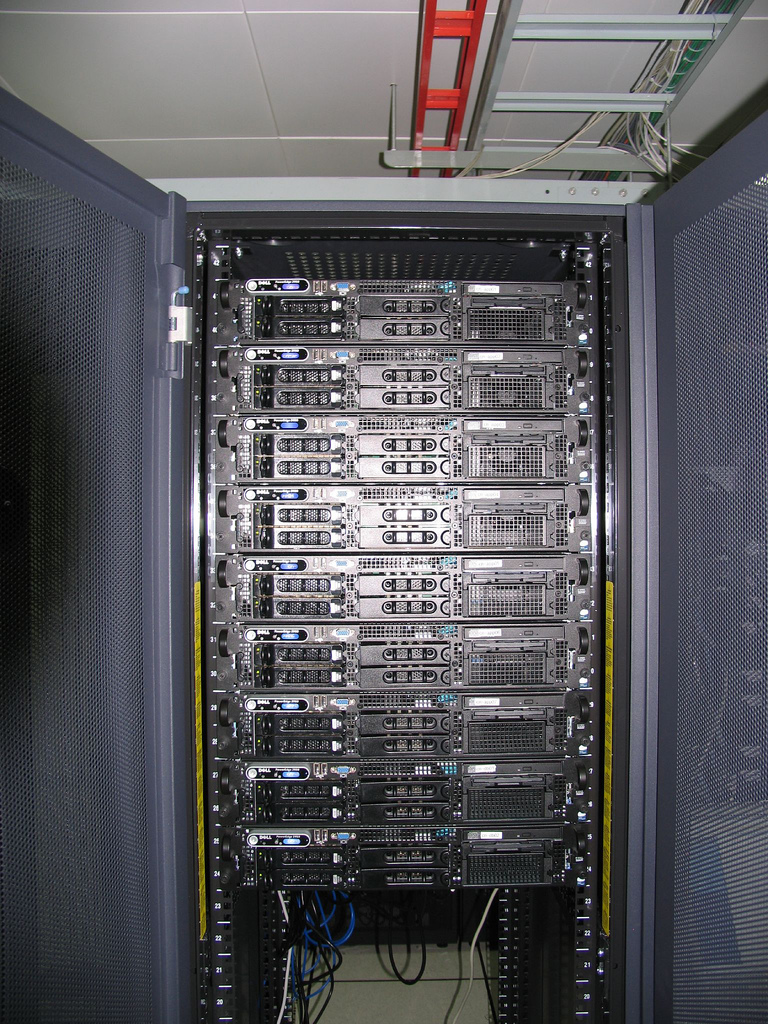
\includegraphics[height=1.5cm]{files/flickr_rack.jpg}
        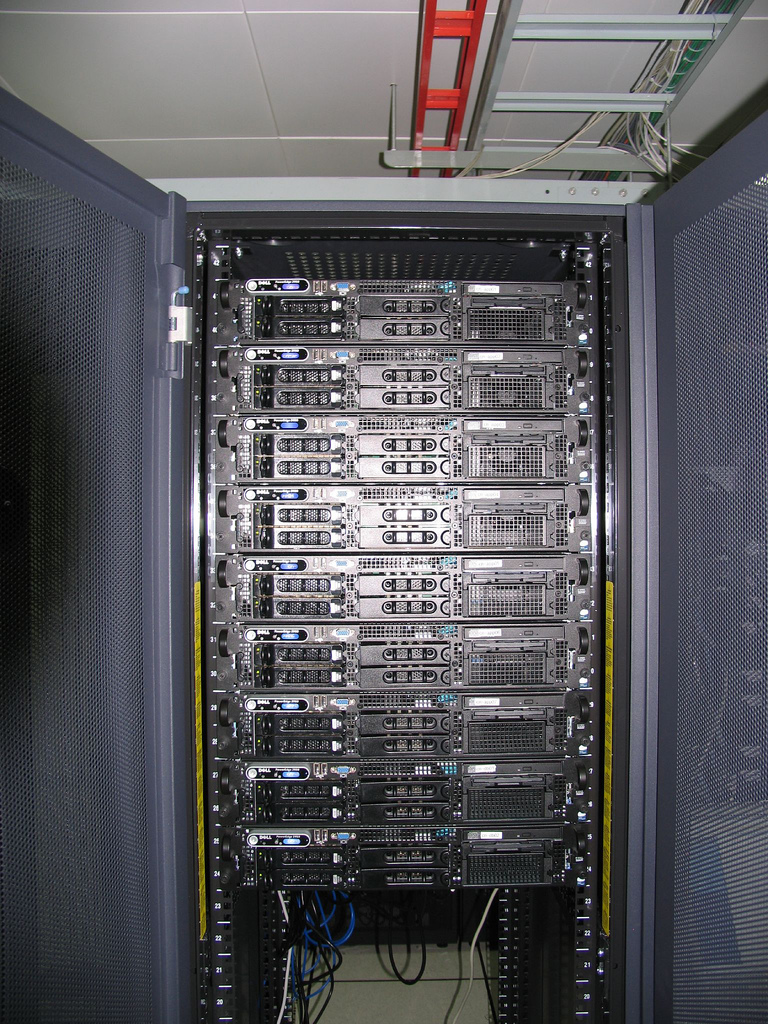
\includegraphics[height=1.5cm]{files/flickr_rack.jpg}
    \end{center}
}

\subsection{Challenges}
\frame{%
\frametitle{Challenges}
    \begin{LARGE}
    \begin{itemize}
        \xitem{Reproducability}
        \xitem{Speed}
        \xitem{Metrics}
        \xitem{Orchestration}
    \end{itemize}
    \end{LARGE}
}
\frame{%
\frametitle{WANTED}

    \flushright{\tiny{\color{darkgrey}http://www.flickr.com/photos/pagedooley/3124443099/}}
    \begin{center}
        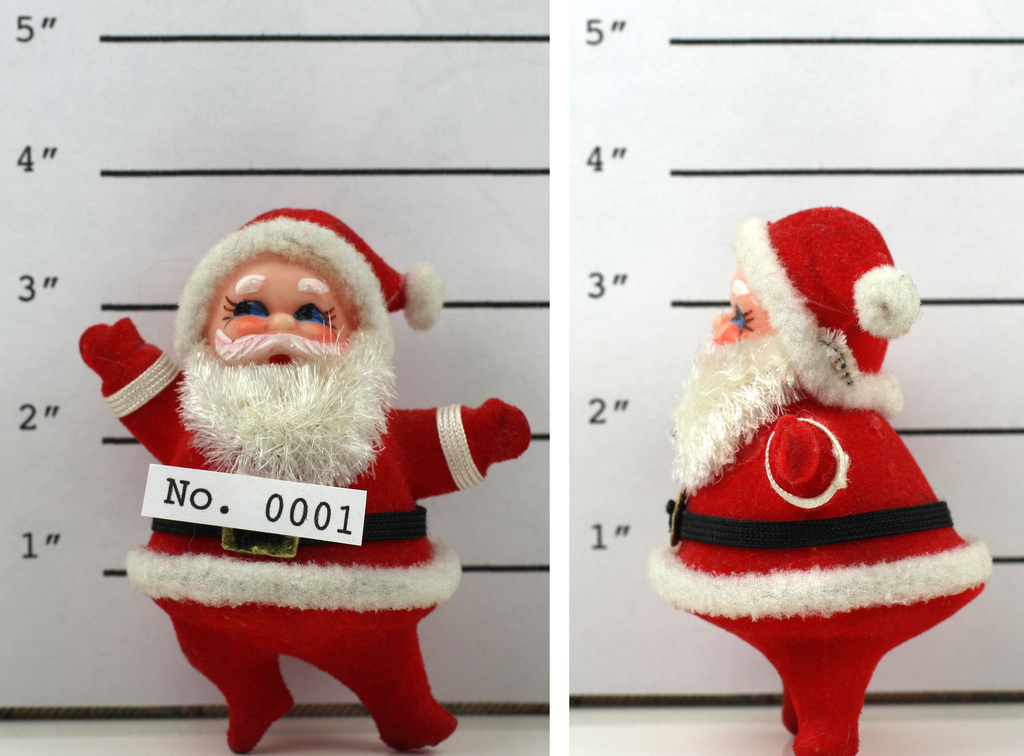
\includegraphics[height=4cm]{files/flickr_wanted.jpg}\\
    \begin{large}
    \begin{itemize}
        \xitem{Small tools}
        \xitem{Collect / Mangle}
        \xitem{Analyse / Act}
        \xitem{Visualize}
    \end{itemize}
    \end{large}
    \end{center}
}
\frame{%
\frametitle{WANTED}

\begin{center}\Huge{\shadowtext{The {\color{inuits}UNIX} philosophy}}\end{center}
}
\subsection{Infrastructure as code}
\frame{%
\frametitle{Automation}

    \begin{LARGE}
    \begin{itemize}
        \xitem{One source of trust: puppet, chef, \ldots}
        \xitem{Exported resource}
        \xitem{Monitor in the same location you deploy}
        \xitem{Infrastructure-as-Code}
        \xitem{\color{inuits}no autodiscovery tools}
    \end{itemize}
    \end{LARGE}
}
\frame{%
\frametitle{Automation}

    \begin{huge}
    \begin{center}
        \shadowtext{If it is not automated || not monitored}\\\shadowtext{then it does not exist!}
    \end{center}
    \end{huge}
}
\frame{%
\frametitle{Example in puppet}
    \begin{large}
    \begin{itemize}
        \xitem{Create a definition for your application}
        \xitem{In that definition, add the configuration, the vhosts\ldots}
        \xitem{Then export the monitoring (@@icinga\_service)}
        \xitem{In bonus you can export DB configuration, etc\ldots}
        \xitem{Use only the "meta" definition}
        \xitem{Collect the exported ressources (Nagios\_service <||>)}
    \end{itemize}
    \end{large}

}
\section{Tools}
\subsection{Collectd}
\frame{%
\frametitle{Collectd}
    \begin{LARGE}
    \begin{itemize}
        \xitem{Statistics collection daemon}
        \xitem{{\color{inuits}A lot} of plugins available\ldots}
        \xitem{Can send data to graphite}
        \xitem{Simple configuration}
    \end{itemize}
    \end{LARGE}
}
\frame{%
\frametitle{Collectd plugins}
    \flushright{\tiny{\color{darkgrey}http://www.flickr.com/photos/juhansonin/3141561416/}}
    \begin{center}
        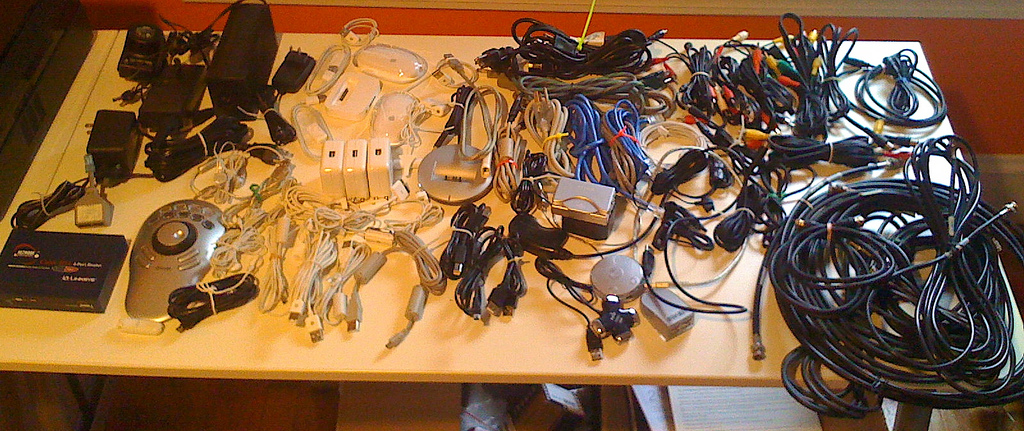
\includegraphics[height=4cm]{files/flickr_plugins.jpg}
    \end{center}
}
\frame{%
\frametitle{Collectd plugins}
\begin{small}
\begin{center}
\shadowtext{AMQP Apache APC\_UPS Apple\_Sensors Ascent Battery BIND Carbon}\\
\shadowtext{ConnTrack ContextSwitch CPU CPUFreq CSV cURL cURL-JSON cURL-XML}\\
\shadowtext{DBI DF Disk DNS E-Mail Entropy Exec FileCount FSCache GenericJMX}\\
\shadowtext{gmond HDDTemp Interface IPMI IPTables IPVS IRQ Java libvirt Load}\\
\shadowtext{LogFile LPAR MadWifi MBMon memcachec memcached Memory Modbus}\\
\shadowtext{Monitorus Multimeter MySQL NetApp Netlink Network NFS nginx}\\
\shadowtext{Notify\_Desktop Notify\_Email NTPd NUT olsrd OneWire OpenVPN OpenVZ}\\
\shadowtext{Oracle Perl Pinba Ping PostgreSQL PowerDNS Processes Protocols Python}\\
\shadowtext{Redis RouterOS RRDCacheD RRDtool Sensors Serial SNMP Swap SysLog}\\
\shadowtext{Table Tail Tape TCPConns TeamSpeak2 TED thermal TokyoTyrant UnixSock}\\
\shadowtext{Uptime Users UUID Varnish vmem VServer Wireless XMMS}\\
\shadowtext{Write\_Graphite Write\_HTTP Write\_MongoDB}\\
\shadowtext{Write\_Redis Write\_Riemann ZFS\_ARC}
\end{center}
\end{small}
}
\subsection{Logstash}
\frame{%
\frametitle{Logstash}
    \begin{LARGE}
    \begin{itemize}
        \xitem{Ship logs from any source}
        \xitem{Filter them}
        \xitem{Index them}
        \xitem{Search them}
        \xitem{Backed with elasticsearch}
    \end{itemize}
    \end{LARGE}
}
\frame{%
\frametitle{Kibana}
    \flushright{\tiny{\color{darkgrey}http://kibana.org/images/screenshots/searchss.png}}
    \begin{center}
    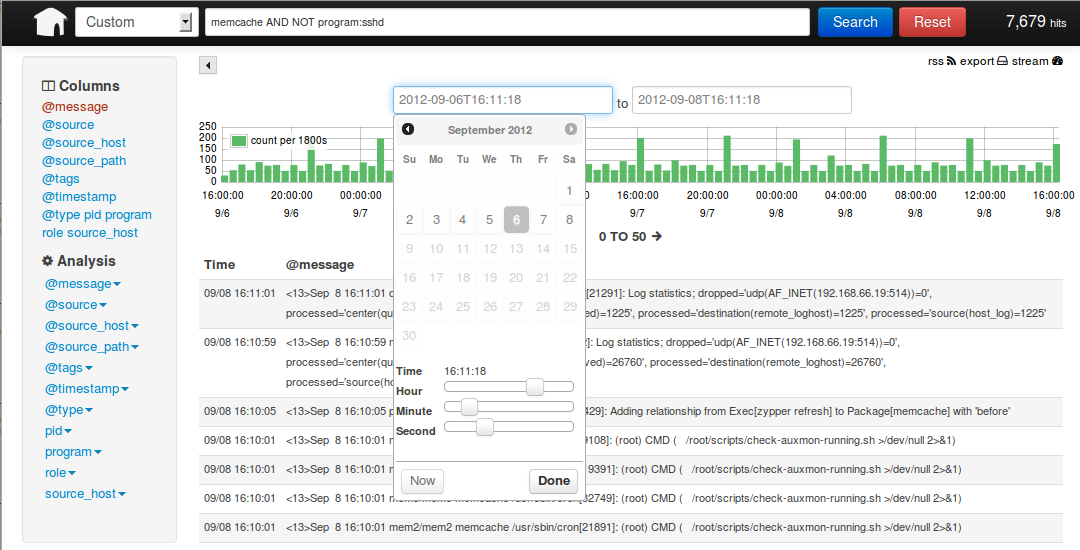
\includegraphics[height=5cm]{files/kibana.png}
    \end{center}
}
\subsection{Statsd}
\frame{%
\frametitle{Statsd}
    \begin{LARGE}
    \begin{itemize}
        \xitem{Stats aggregation}
        \xitem{Simple counters}
        \xitem{Flushes every XX seconds to graphite}
        \xitem{Text over UDP}
    \end{itemize}
    \end{LARGE}
}
\frame{%
\frametitle{Statsd}
    \begin{center}
        \small{\shadowtext{echo "stats.sshd.login:1|c" | nc -u statsd.example.com 8125}}
    \end{center}
}
\subsection{Graphite}
\frame{%
\frametitle{Graphite}
    \begin{LARGE}
    \begin{itemize}
        \xitem{Graphing made simple}
        \xitem{A lot of helpers functions}
        \xitem{Listening on UDP and TCP}
        \xitem{Text over UDP/TCP}
    \end{itemize}
    \end{LARGE}
}
\frame{%
\frametitle{Send data to graphite}
        \small{\shadowtext{echo "stats.sshd.login 1 \$(date +\%s)" | nc -u graphite.example.com 2003}}
}
\frame{%
\frametitle{Graphite API}
    \begin{center}
    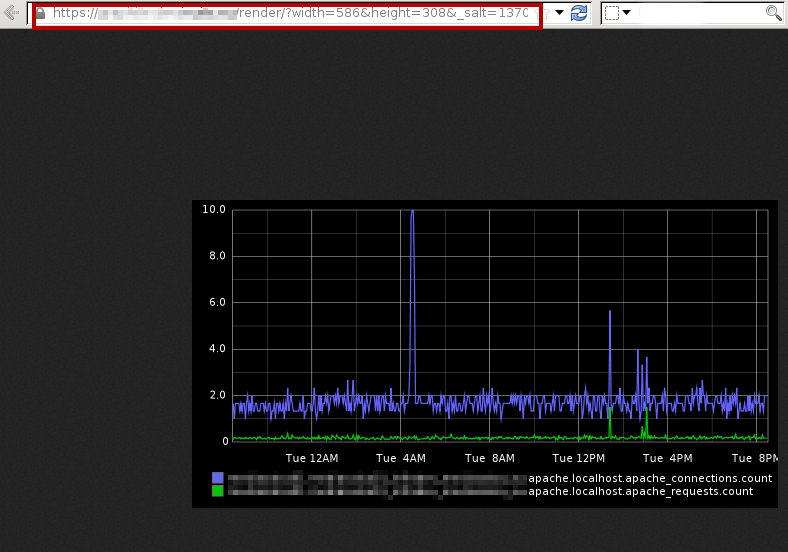
\includegraphics[height=5cm]{files/graphite-api.png}
    \end{center}

}

\frame{%
\frametitle{gdash}

    \flushright{\tiny{\color{darkgrey}https://github.com/ripienaar/gdash}}
    \begin{center}
    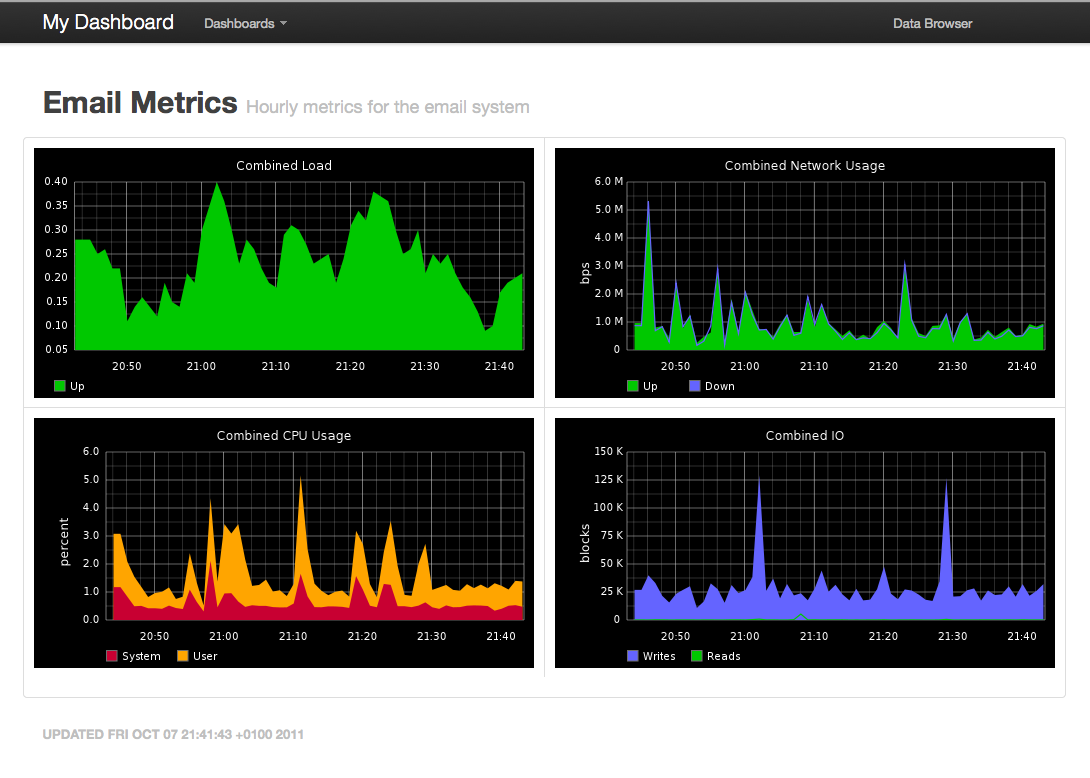
\includegraphics[height=5cm]{files/gdash.png}
    \end{center}

}
\subsection{Icinga}
\frame{%
\frametitle{Icinga}
    \begin{LARGE}
    \begin{itemize}
        \xitem{Fork of nagios}
        \xitem{Large and vibrant community}
        \xitem{Configuration compatible with nagios}
        \xitem{User-friendly interface}
        \xitem{\color{inuits}Use Icinga Classic!}
    \end{itemize}
    \end{LARGE}
}
\frame{%
\frametitle{Icinga}
    \flushright{\tiny{\color{darkgrey}https://icinga.org}}
    \begin{center}
    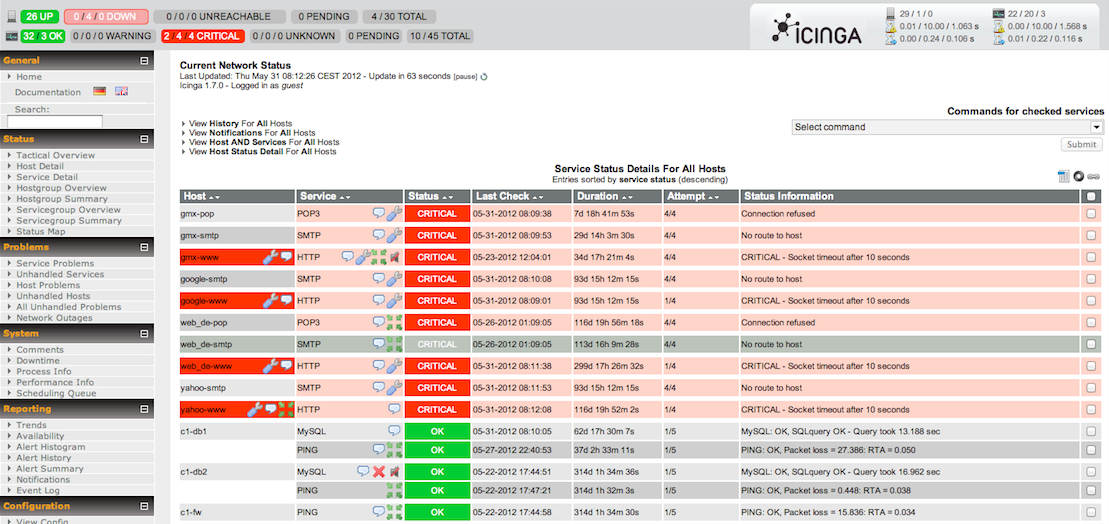
\includegraphics[height=5cm]{files/Icinga_Classic_ServiceStatus.png}
    \end{center}

}
\section{Conclusion}
\subsection{They work together}
\frame{%
\frametitle{Toolchain from apache to nagios}
    \begin{large}
    \begin{itemize}
        \xitem{Apache ships logs to rsyslog}
        \xitem{Rsyslog ships logs to logstash}
        \xitem{Logstash ships metrics to statsd}
        \xitem{Statsd ships metrics to Graphite}
        \xitem{Icinga query metric from graphite}
        \xitem{https://github.com/etsy/nagios\_tools}
    \end{itemize}
    \end{large}
}
\frame{%
\frametitle{Reusing Icinga/Nagios perfdata}
    \begin{large}
    \begin{itemize}
        \xitem{Icinga performs various checks}
        \xitem{Icinga sends perfdata to graphite}
        \xitem{Graphite stores the data}
        \xitem{Gdash serves them inside dashboards}
        \xitem{https://github.com/roidelapluie/icinga-to-graphite}
    \end{itemize}
    \end{large}
}
\subsection{Sharing}
\frame{%
\frametitle{The metrics}
    \begin{LARGE}
    \begin{itemize}
        \xitem{Everything can become a metric}
        \xitem{Performance metrics}
        \xitem{Usage metrics}
        \xitem{Business-valuable metrics}
        \xitem{People metrics}
        \xitem{Metrics are knowledge}
    \end{itemize}
    \end{LARGE}
}
\frame{%
\frametitle{Metrics that matter}
    \flushright{\tiny{\color{darkgrey}http://codeascraft.com/2011/02/15/measure-anything-measure-everything/}}
    \begin{center}
    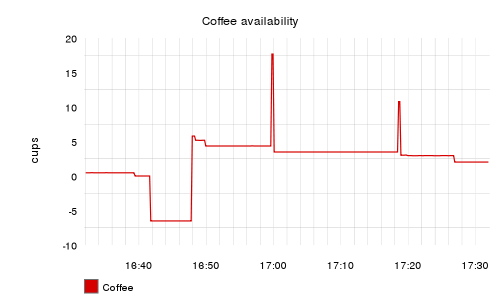
\includegraphics[height=5cm]{files/coffee.png}
    \end{center}
}
\subsection{There are solutions}
\frame{%
\frametitle{What have we seen?}
    \begin{LARGE}
    \begin{itemize}
        \xitem{We have seen only open-source software}
        \xitem{Small, pluggable daemons}
        \xitem{Robust solutions}
        \xitem{Nice \& user-friendly output}
        \xitem{They play together}
    \end{itemize}
    \end{LARGE}
}
\frame{%
\frametitle{Homework}
    \begin{large}
    \begin{itemize}
        \xitem{Sensu}
        \xitem{Riemann}
        \xitem{Extremon}
        \xitem{Esper}
        \xitem{Skyline}
        \xitem{Oculus}
    \end{itemize}
    \end{large}
}
\frame{%
\frametitle{Try them yourself}
    \begin{large}
    \shadowtext{https://github.com/KrisBuytaert/vagrant-graphite}\\
    \shadowtext{https://github.com/KrisBuytaert/vagrant-puppet-logstash}
    \end{large}
}
\frame{%
\frametitle{Contact}
    \begin{columns}[T]
        \begin{column}{.5\textwidth}
    \begin{large}
    \shadowtext{Julien Pivotto}\\
    \shadowtext{julien@inuits.eu}\\
    \shadowtext{@roidelapluie}
    \end{large}
        \end{column}
        \begin{column}{.5\textwidth}
    \vspace{2cm}
    \begin{small}
    
\includegraphics[height=2cm]{files/inuitslogo.png}\\
    \shadowtext{INUITS bvba}\\
    \shadowtext{Duboisstraat 50}\\
    \shadowtext{2060 Antwerp}\\
    \shadowtext{Belgium}\\
    \shadowtext{+32 473 441 636}\\
    \shadowtext{https://inuits.eu}
    \end{small}
        \end{column}
        \end{columns}
}






\end{document}
